\section{Observations}

\subsection*{Observational Data}

    % \subsubsection{For Air}

        % \paragraph*{Measurement of charge $Q$ for different supply voltage $U_c$}

            \begin{table}[H]
    \centering
    \begin{tabular}{|c|c|c|}
    \hline
    $U_c$ (kV)& $V_o$ (V) & $Q$ (nAs) \\ \hline
    0.5 & 0.68  &  149.6 \\
     1.0 & 1.28  &  281.6 \\
     1.5 & 1.73 &  379.5 \\
     2.0 & 2.13 &  467.5 \\
     2.5 & 2.68 &  588.5 \\
     3.0 & 3.50  &  770.0   \\
     3.5 & 3.95  &  869.0   \\
     4.0 & 4.55  & 1001.0   \\
    \hline
    \end{tabular}
    \caption{$Q$ vs $U_C$ data with air as the dielectric medium}
    \label{tab:1}
\end{table}

        % \paragraph*{Measurement of charge $Q$ for different distances $d$}

        \begin{table}[H]
    \centering
    \begin{tabular}{|c|c|c|}
    \hline
        $d$ (mm)& $V_o$ (V) & $Q$ (nAs) \\ \hline
        1.0 & 3.8 & 836 \\
        1.5 & 2.6 & 572 \\
        2.0 & 2.0 & 440 \\
        2.5 & 1.5 & 330 \\
        3.0 & 1.3 & 286 \\
        3.5 & 1.1 & 242 \\
        4.0 & 1.0 & 220 \\
    \hline
    \end{tabular}
    \caption{$Q$ vs $d$ data with air as the dielectric medium}
    \label{tab:2}
\end{table}

    % \subsubsection{For Styrofoam}
        \begin{table}[H]
    \centering
    \begin{tabular}{|c|c|c|}
    \hline
        $U_c$ (kV)& $V_o$ (V) & $Q$ (nAs) \\ \hline
        0.5 & 0.136 &  30.066 \\
        1.0 & 0.246 &  54.266 \\
        1.5 & 0.373 &  82.133 \\
        2.0 & 0.503 & 110.733  \\
        2.5 & 0.633 & 139.333  \\
        3.0 & 0.736 & 162.067  \\
        3.5 & 0.873 & 192.133  \\
        4.0 & 0.973 & 214.133  \\
    \hline
    \end{tabular}
    \caption{$Q$ vs $U_c$ data with styrofoam as the dielectric medium}
    \label{tab:3}
\end{table}

    % \subsubsection{For Wood}
        \begin{table}[H]
    \centering
    \begin{tabular}{|c|c|c|}
    \hline
        $U_c$ (kV)& $V_o$ (V) & $Q$ (nAs) \\ \hline
        0.5 & 1.4     &  308     \\
    1.0 & 1.9 &  425 \\
    1.5 & 2.4 &  542\\
    2.0 & 2.9 &  652 \\
    2.5 & 3.5     &  770     \\
    3.0 & 3.9 &  872 \\
    3.5 & 4.3     &  946     \\
    4.0 & 4.6     & 1012     \\
    \hline
    \end{tabular}
    \caption{$Q$ vs $U_C$ data with wood as the dielectric medium}
    \label{tab:4}
\end{table}


\subsection*{Calculations}
    For all the calculations, we take $\varepsilon_o = 8.854\cross10^{-12}$ F/m and $A = \pi(13)^2 \text{cm}^2 = 5.31\cross10^{-2}$ m$^2$\\

    \begin{enumerate}
        \item \textbf{Measurement of $\varepsilon_\text{air}$ from $Q \sim U_c$ data}
            \begin{figure}[H]
                \centering
                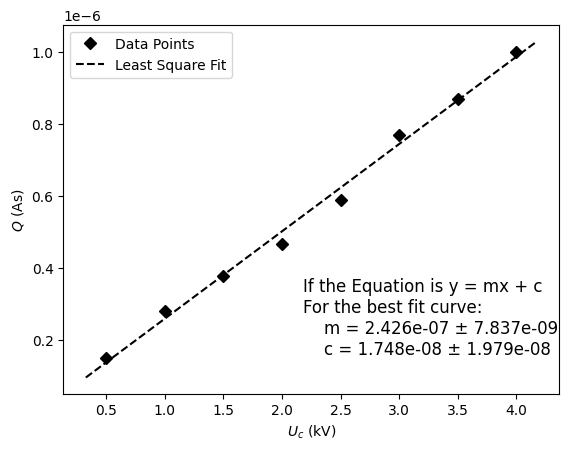
\includegraphics[width=0.8\columnwidth]{images/g1.png}
                \caption{$Q$ vs $U_C$ plot with air as the dielectric medium}
                \label{g1}
            \end{figure}

            From Fig. \ref{g1}, slope $=2.426 \cross 10^{-10}$ As/V. From eq. (12), we get,
                
            \begin{align*}
                \varepsilon_\text{air}^{a} &= \frac{d}{\varepsilon_oA} \cdot \text{slope}=1.032
            \end{align*}
            
            where $d=2$ mm.\\

        \item \textbf{Measurement of $\varepsilon_\text{air}$ from $Q \sim d^{-1}$ data}
            \begin{figure}[H]
                \centering
                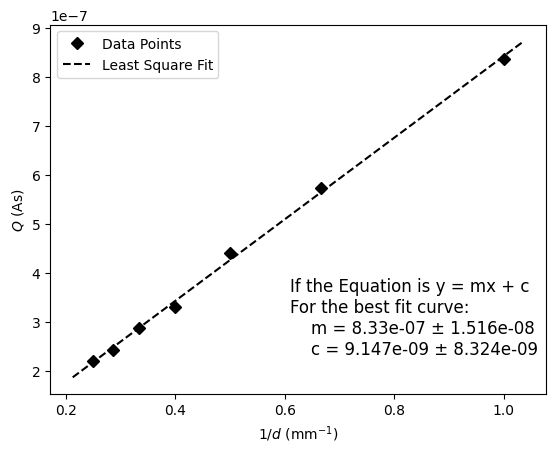
\includegraphics[width=0.8\columnwidth]{images/g2.png}
                \caption{$Q$ vs $d$ data with air as the dielectric medium}
                \label{g2}
            \end{figure}

            From Fig. \ref{g2}, slope $=8.33 \cross 10^{-10}$ As/V. Rearranging eq. (12) to keep $U_c$ constant and vary $d$, we get,
                
            \begin{align*}
                \varepsilon_\text{air}^{b} &= \frac{\text{slope}}{\varepsilon_oAU_c} \cdot =1.181
            \end{align*}
            
            where $U_c=1.5$ kV.

            From $\varepsilon_\text{air}^a$ and $\varepsilon_\text{air}^b$, we can calculate the mean value of $\varepsilon_\text{air}=1.106$.\\

        \item \textbf{Measurement of $\varepsilon_\text{styrofoam}$ from $Q \sim U_c$ data}
            \begin{figure}[H]
                \centering
                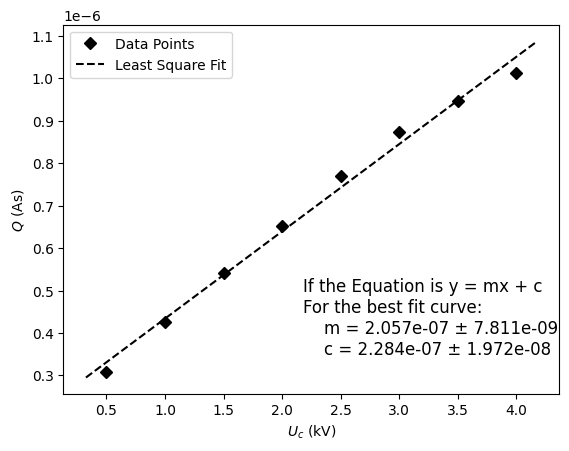
\includegraphics[width=0.8\columnwidth]{images/g3.png}
                \caption{$Q$ vs $U_c$ data with styrofoam as the dielectric medium}
                \label{g3}
            \end{figure}

            From Fig. \ref{g3}, slope $=5.348 \cross 10^{-11}$ As/V. From eq. (12), we get,
                
            \begin{align*}
                \varepsilon_\text{styrofoam} &= \frac{d}{\varepsilon_oA} \cdot \text{slope}=2.184
            \end{align*}
            
            where $d=19.2$ mm.\\

        \item \textbf{Measurement of $\varepsilon_\text{wood}$ from $Q \sim U_c$ data}
            \begin{figure}[H]
                \centering
                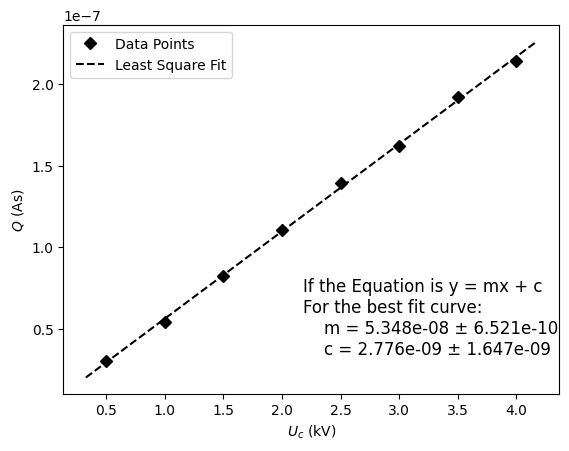
\includegraphics[width=0.8\columnwidth]{images/g4.png}
                \caption{$Q$ vs $U_c$ data with wood as the dielectric medium}
                \label{g4}
            \end{figure}

            From Fig. \ref{g4}, $=2.057 \cross 10^{-10}$ As/V. From eq. (12), we get,
                
            \begin{align*}
                \varepsilon_\text{wood} &= \frac{d}{\varepsilon_oA} \cdot \text{slope}=3.588
            \end{align*}
            
            where $d=8.2$ mm.

    \end{enumerate}


